\documentclass[10pt,landscape]{article}
\usepackage{multicol}
\usepackage{calc}
\usepackage{ifthen}
\usepackage[landscape]{geometry}
\usepackage{amsmath,amsthm,amsfonts,amssymb}
\usepackage{color,graphicx,overpic}
\usepackage{hyperref}
\usepackage{listings}
% My Environments
\usepackage[breakable]{tcolorbox}

\usepackage{graphicx}
\lstset{
  basicstyle=\ttfamily,
  columns=fullflexible,
  frame=single,
  breaklines=true,
  postbreak=\mbox{\textcolor{red}{$\hookrightarrow$}\space},
}

\pdfinfo{
  /Title (example.pdf)
  /Creator (TeX)
  /Producer (pdfTeX 1.40.0)
  /Author (Seamus)
  /Subject (Example)
  /Keywords (pdflatex, latex,pdftex,tex)}

% This sets page margins to .5 inch if using letter paper, and to 1cm
% if using A4 paper. (This probably isn't strictly necessary.)
% If using another size paper, use default 1cm margins.
\ifthenelse{\lengthtest { \paperwidth = 11in}}
    { \geometry{top=.5in,left=.5in,right=.5in,bottom=.5in} }
    {\ifthenelse{ \lengthtest{ \paperwidth = 297mm}}
        {\geometry{top=1cm,left=1cm,right=1cm,bottom=1cm} }
        {\geometry{top=1cm,left=1cm,right=1cm,bottom=1cm} }
    }

% Turn off header and footer
\pagestyle{empty}

% Redefine section commands to use less space
\makeatletter
\renewcommand{\section}{\@startsection{section}{1}{0mm}%
                                {-1ex plus -.5ex minus -.2ex}%
                                {0.5ex plus .2ex}%x
                                {\normalfont\large\bfseries}}
\renewcommand{\subsection}{\@startsection{subsection}{2}{0mm}%
                                {-1explus -.5ex minus -.2ex}%
                                {0.5ex plus .2ex}%
                                {\normalfont\normalsize\bfseries}}
\renewcommand{\subsubsection}{\@startsection{subsubsection}{3}{0mm}%
                                {-1ex plus -.5ex minus -.2ex}%
                                {1ex plus .2ex}%
                                {\normalfont\small\bfseries}}
\makeatother

% Define BibTeX command
\def\BibTeX{{\rm B\kern-.05em{\sc i\kern-.025em b}\kern-.08em
    T\kern-.1667em\lower.7ex\hbox{E}\kern-.125emX}}

% Don't print section numbers
\setcounter{secnumdepth}{0}


\setlength{\parindent}{0pt}
\setlength{\parskip}{0pt plus 0.5ex}

%My Environments
\newtheorem{example}[section]{Example}
% -----------------------------------------------------------------------

\begin{document}
\raggedright
\footnotesize
\begin{multicols}{3}


    % multicol parameters
    % These lengths are set only within the two main columns
    %\setlength{\columnseprule}{0.25pt}
    \setlength{\premulticols}{1pt}
    \setlength{\postmulticols}{1pt}
    \setlength{\multicolsep}{1pt}
    \setlength{\columnsep}{2pt}

    \begin{center}
        \Large{\underline{CHE374}} \\
    \end{center}

    \section{Cheat Sheet}
    Relevant: Weeks 1 - 8

    \subsection{Week 1 - Time Value of Money}
    \begin{tcolorbox}[boxsep=0pt, left=0pt, right=0pt, top=0pt, bottom=0pt]
        \begin{tabular}{p{2cm} p{5cm}}
            Future Value                 & $F = P(1+i)$                                                                                                                                                     \\
            Simple Interest              & $F_N = P(1 + iN)$                                                                                                                                                \\
            Compound \linebreak Interest & $F = P(1 + i)^N$                                                                                                                                                 \\
            Subperiod Compounding        & $F = P(1 + \frac{r}{m})^{mN}$                                                                                                                                    \\
            Eff. Annual Interest Rate    & $i_{e} = (1 + \frac{r} {m})^m - 1 = (\frac{F}{P})^{\frac{12}{N}} - 1 $\linebreak Eq. 2, only T-bills                                                             \\
            Continuously Compounding     & $i_e =\lim\limits_{m \to \infty} (1 + \frac{r}{m})^m- 1 = e^r - 1$                                                                                               \\
            Continuous Compounding       & $r =\lim\limits_{m \to \infty} ((i_e + 1) - 1)m = \ln(1 + i_e)$                                                                                                  \\
            Future Interest Rates        & \smash{\scalebox{1}{$(1 + r_{1, x})^{\frac{x}{12}} = (1 + r_{1, k})^{\frac{k}{12}} (1 + r_{k, x})^{\frac{x-k}{12}}$}} $r_{a,b}$ is the rate from time $a$ to $b$ \\
        \end{tabular}
    \end{tcolorbox}
    \section{Week 2 - Cash-flow Analysis}
    \begin{tcolorbox}[boxsep=0pt, left=0pt, right=0pt, top=0pt, bottom=0pt]
        \begin{tabular}{p{2cm} p{5cm}}
            Arithmetic Gradient & $A_n = A' + (N-1)G$ $A'$: the original, $G$: amnt added, $N$: \# of periods           \\
            Geometric Gradient  & $A_n = A'(1 + g)^{N-1}$                                                               \\
            Compound Amount     & \smash{\scalebox{0.95}{$(F/P, i, N) = (1 + i)^N, (P/F, i, N) = \frac{1}{(1 + i)^N}$}} \\
            Perpetuity          & $(P/A, i) = \frac{1}{i},\quad (A/P, i) = i$                                           \\
            Annuity             & $(P/A, i, N) = \frac{1}{i}(1 - \frac{1}{(1 + i)^N})$                                  \\
            Arithmetic Growth   & $(P/G, i, N) = \frac{1}{i^2}\left(1 - \frac{1+iN}{(1 + i)^N}\right)$                  \\
            Geometric Growth    & $(P/G, i, g, N) = \frac{1 - (\frac{1 + g}{1 + i})^N}{i - g}$                          \\
        \end{tabular}
    \end{tcolorbox}
    \section{Week 3 - Mortgages and Bonds}

    \begin{tcolorbox}[boxsep=0pt, left=0pt, right=0pt, top=0pt, bottom=0pt]
        \begin{tabular}{p{2cm} p{5cm}}
            Loan to Value Ratio  & $LTV = \frac{Principle}{House Value}$                                                  \\
            Ammortization Period & \# of years it takes to pay off the loan.                                              \\
            Mortgage Term        & \# of years the interest rate is fixed,\linebreak after which the rate is renegotiated \\
            Face/Par Value       & Value received at bond maturity                                                        \\
            Coupon Rate          & Interest rate paid annually on the bond                                                \\
        \end{tabular}
    \end{tcolorbox}
    \section{Week 4 - Risk, Reward, and Arbitrage}
    \begin{tcolorbox}[boxsep=0pt, left=0pt, right=0pt, top=0pt, bottom=0pt]
        \begin{tabular}{p{2cm} p{5cm}}
            Return vector              & $\overrightarrow{R_i}=\begin{bmatrix}r_{t_1}\\\vdots\\ r_{t_n} \end{bmatrix}, \quad r_{t_{j}} = \frac{1}{\Delta t} \ln\left(\frac{P_{t_j}}{P_{t_{j-1}}}\right)$ \linebreak A portfolio of $n$ stocks, the returns of project $i$ at $t_j$ \\
            Volatility                 & \smash{\scalebox{1}{$\sigma = \sqrt{Var(\overrightarrow{R_i})} = \sqrt{\frac{1}{n-1} \sum_{i=1}^{n} (r_i - \bar{r})^2}$}}                                                                                                                 \\
            Average\linebreak Return   & $\bar{r} = \frac{1}{n} \sum_{i=1}^{n} r_i$                                                                                                                                                                                                \\
            Covariance                 & \smash{\scalebox{0.95}{$Cov(\overrightarrow{R_i},\overrightarrow{R_j}) = \frac{1}{n-1} \sum_{i=1}^{n} (r_{i} - \bar{r_i})(r_{j} - \bar{r_j})$}}                                                                                           \\
            Covariance Matrix          & $        \Sigma = \begin{bmatrix}
                                                                   \sigma_{11} & \sigma_{12} & \cdots & \sigma_{1n} \\
                                                                   \sigma_{21} & \sigma_{22} & \cdots & \sigma_{2n} \\
                                                                   \vdots      & \vdots      & \ddots & \vdots      \\
                                                                   \sigma_{n1} & \sigma_{n2} & \cdots & \sigma_{nn}
                                                               \end{bmatrix}$                                                                                                                                                                        \\
            Covariances                & $\sigma_{ij} = \sigma_{ji} = Cov(\overrightarrow{R_i},\overrightarrow{R_j})$                                                                                                                                                              \\
                                       & $\sigma_{ii} = Var(\overrightarrow{R_i})$                                                                                                                                                                                                 \\
            Portfolio                  & $\overrightarrow{X} = \begin{bmatrix}
                                                                       x_1    \\
                                                                       \vdots \\n
                                                                       x_n
                                                                   \end{bmatrix}$ We invest $x_i$ in each stock.                                                                                                                                                                       \\
            Portfolio\linebreak Return & $\mathbb{E}[\overrightarrow{R_p}] = \sum_{i=1}^{n} x_i \mathbb{E}[\overrightarrow{R_i}]$                                                                                                                                                  \\
            Portfolio Volatility       & $\sigma_p = \sqrt{\overrightarrow{X}^T \times \Sigma \times \overrightarrow{X}}$                                                                                                                                                          \\
            \multicolumn{2}{c}{CAPM Assumptions}                                                                                                                                                                                                                                   \\
            \multicolumn{2}{c}{\begin{minipage}{7.5cm}
                                       \begin{itemize}
                        \item Correlation \& volatility of/between assets are fixed
                        \item Investors aim to make as much money as possible
                        \item Investors are rational and risk-averse
                        \item Investors have the same info at the same time
                        \item Investors have accurate conception of possible returns, i.e. the probability beliefs of investors match the true distribution of returns.
                        \item No taxes or transaction costs
                        \item Actions of investors do not influence prices
                        \item Investors can lend and borrow unlimited amounts at the risk free rate
                        \item Securities can be divided into any size
                    \end{itemize}
                                   \end{minipage}}                                                                                                                                                                                                                            \\
            \multicolumn{2}{c}{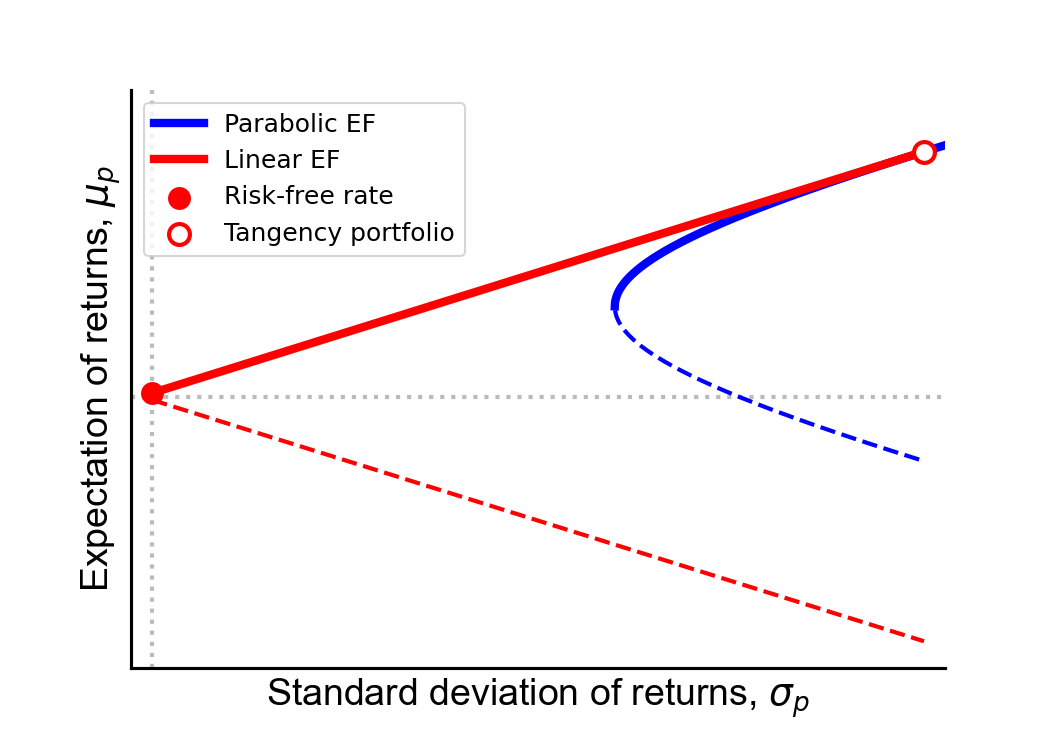
\includegraphics[width=0.6\textwidth]{LECTURE_4/CML.png}}                                                                                                                                                                                           \\
            \multicolumn{2}{c}{Efficiency Frontier \& Capital Market Line}                                                                                                                                                                                                         \\
            \multicolumn{2}{l}{Minimize $\sigma_p^2 = \overrightarrow{X}^T \Sigma \overrightarrow{X}$}                                                                                                                                                                             \\
            \multicolumn{2}{l}{While $\sum_{i=1}^{n} x_i = 1, \, \sum_{i=1}^{n} x_i \mathbb{E}[R_i] = \mathbb{E}[R_p],\, \sum_{i=1}^{n} x_i \sigma_i = \sigma_p$}
        \end{tabular}
    \end{tcolorbox}
    \section{Week 4 - Contd.}
    \begin{tcolorbox}[boxsep=0pt, left=0pt, right=0pt, top=0pt, bottom=0pt]
        \begin{tabular}{p{2cm} p{5cm}}
            Leveraging                & $\mathbb{E}[R_{p}] = w\cdot \mathbb{E}[R_{m}] + (1-w)\cdot r_f \quad w$ is the weight of MP                            \\
                                      & $\sigma_{p} = \sqrt{w^2 \sigma_{m}^2 + (1-w)^2 \cdot \sigma_{f}}, \,\, \sigma_{f} = 0$                                 \\
            Systematic Risk           & $\beta_i = \frac{Cov(R_i,R_m)}{Var(R_m)} = \frac{\sigma_{i,m}}{\sigma_{m}^2} = \frac{\rho_{i,m} \sigma_i}{\sigma_{m}}$ \\
            Asset Expected Return     & $\mathbb{E}[R_i] = r_f + \beta_i(\mathbb{E}[R_m] - r_f)$                                                               \\
            \multicolumn{2}{c}{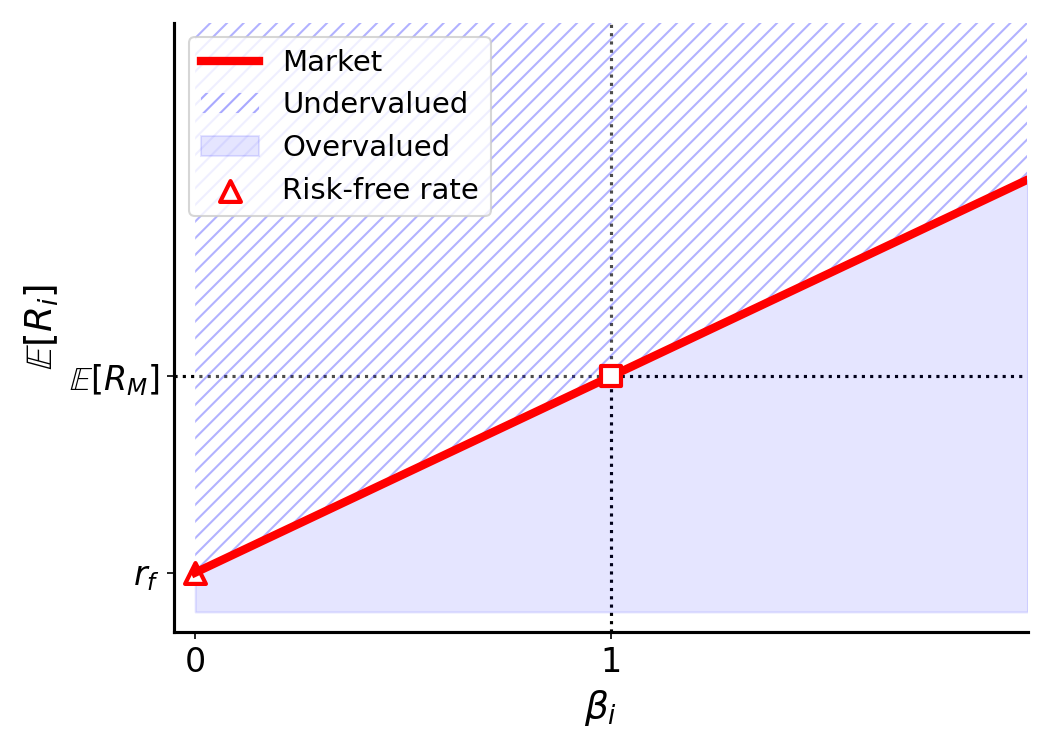
\includegraphics[width=0.6\textwidth]{LECTURE_4/SML.png}}                                                                       \\
            \multicolumn{2}{c}{Security Market Line (Asset Expected Return Plotted)}                                                                           \\
            Forwards/Futures          & Contract to buy/sell assets at a future date at a price agreed upon today                                              \\
            Expected Value            & $\mathbb{E}[P] = \sum_{i=1}^{n} P_i \cdot p_i$                                                                         \\
                                      & $p_i$ is the probability of $P_i$ occurring                                                                            \\
            Expected\linebreak Return & $\mathbb{E}[R] = \frac{\mathbb{E}[P]}{P_0} -1 = \frac{\sum_{i=1}^{n} P_i \cdot p_i}{P_0} -1$
        \end{tabular}
    \end{tcolorbox}
    \section{Week 5 - Comparison Methods 1}
    \begin{tcolorbox}[boxsep=0pt, left=0pt, right=0pt, top=0pt, bottom=0pt]
        \begin{tabular}{p{2cm} p{5cm}}
            MARR          & Interest on the best alternative \\
            Present Worth &
        \end{tabular}
    \end{tcolorbox}
\end{multicols}
\end{document}